%\documentclass[tikz]{standalone}

%\begin{document}

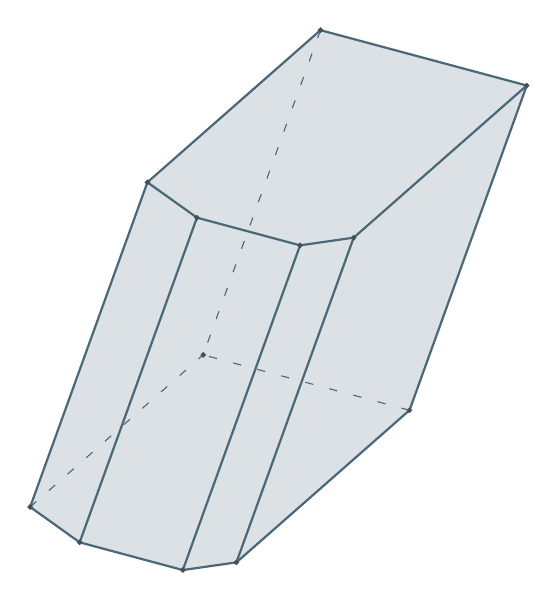
\begin{tikzpicture}%
	[x={(0.907792cm, 0.130012cm)},
	y={(-0.419345cm, 0.299380cm)},
	z={(0.007956cm, 0.945234cm)},
	scale=.015,
	back/.style={loosely dashed, thin},
	edge/.style={color=cyan!40!black, thick},
	facet/.style={fill=cyan!40!black, fill opacity=0.2},
	vertex/.style={inner sep=0pt,circle,draw=cyan!25!black,fill=cyan!75!black,thick,anchor=base}]
%
%
%% Coordinate of the vertices:
%%
\coordinate (-400.00000, -100.00000, -100.00000) at (-400.00000, -100.00000, -100.00000);
\coordinate (-200.00000, 100.00000, 100.00000) at (-200.00000, 100.00000, 100.00000);
\coordinate (-100.00000, -100.00000, 100.00000) at (-100.00000, -100.00000, 100.00000);
\coordinate (-300.00000, -300.00000, -100.00000) at (-300.00000, -300.00000, -100.00000);
\coordinate (200.00000, 200.00000, 100.00000) at (200.00000, 200.00000, 100.00000);
\coordinate (0.00000, 0.00000, -100.00000) at (0.00000, 0.00000, -100.00000);
\coordinate (100.00000, 400.00000, 100.00000) at (100.00000, 400.00000, 100.00000);
\coordinate (-100.00000, 200.00000, -100.00000) at (-100.00000, 200.00000, -100.00000);
\coordinate (-150.00000, -100.00000, 100.00000) at (-150.00000, -100.00000, 100.00000);
\coordinate (-350.00000, -300.00000, -100.00000) at (-350.00000, -300.00000, -100.00000);
\coordinate (-400.00000, -200.00000, -100.00000) at (-400.00000, -200.00000, -100.00000);
\coordinate (-200.00000, 0.00000, 100.00000) at (-200.00000, 0.00000, 100.00000);
%%
%%
%% Drawing edges in the back
%%
\draw[edge,back] (-400.00000, -100.00000, -100.00000) -- (-100.00000, 200.00000, -100.00000);
\draw[edge,back] (0.00000, 0.00000, -100.00000) -- (-100.00000, 200.00000, -100.00000);
\draw[edge,back] (100.00000, 400.00000, 100.00000) -- (-100.00000, 200.00000, -100.00000);
%%
%%
%% Drawing vertices in the back
%%
\node[vertex] at (-100.00000, 200.00000, -100.00000)     {};
%%
%%
%% Drawing the facets
%%
\fill[facet] (-200.00000, 0.00000, 100.00000) -- (-150.00000, -100.00000, 100.00000) -- (-350.00000, -300.00000, -100.00000) -- (-400.00000, -200.00000, -100.00000) -- cycle {};
\fill[facet] (-200.00000, 0.00000, 100.00000) -- (-200.00000, 100.00000, 100.00000) -- (-400.00000, -100.00000, -100.00000) -- (-400.00000, -200.00000, -100.00000) -- cycle {};
\fill[facet] (-350.00000, -300.00000, -100.00000) -- (-300.00000, -300.00000, -100.00000) -- (-100.00000, -100.00000, 100.00000) -- (-150.00000, -100.00000, 100.00000) -- cycle {};
\fill[facet] (0.00000, 0.00000, -100.00000) -- (-300.00000, -300.00000, -100.00000) -- (-100.00000, -100.00000, 100.00000) -- (200.00000, 200.00000, 100.00000) -- cycle {};
\fill[facet] (-200.00000, 0.00000, 100.00000) -- (-200.00000, 100.00000, 100.00000) -- (100.00000, 400.00000, 100.00000) -- (200.00000, 200.00000, 100.00000) -- (-100.00000, -100.00000, 100.00000) -- (-150.00000, -100.00000, 100.00000) -- cycle {};
%%
%%
%% Drawing edges in the front
%%
\draw[edge] (-400.00000, -100.00000, -100.00000) -- (-200.00000, 100.00000, 100.00000);
\draw[edge] (-400.00000, -100.00000, -100.00000) -- (-400.00000, -200.00000, -100.00000);
\draw[edge] (-200.00000, 100.00000, 100.00000) -- (100.00000, 400.00000, 100.00000);
\draw[edge] (-200.00000, 100.00000, 100.00000) -- (-200.00000, 0.00000, 100.00000);
\draw[edge] (-100.00000, -100.00000, 100.00000) -- (-300.00000, -300.00000, -100.00000);
\draw[edge] (-100.00000, -100.00000, 100.00000) -- (200.00000, 200.00000, 100.00000);
\draw[edge] (-100.00000, -100.00000, 100.00000) -- (-150.00000, -100.00000, 100.00000);
\draw[edge] (-300.00000, -300.00000, -100.00000) -- (0.00000, 0.00000, -100.00000);
\draw[edge] (-300.00000, -300.00000, -100.00000) -- (-350.00000, -300.00000, -100.00000);
\draw[edge] (200.00000, 200.00000, 100.00000) -- (0.00000, 0.00000, -100.00000);
\draw[edge] (200.00000, 200.00000, 100.00000) -- (100.00000, 400.00000, 100.00000);
\draw[edge] (-150.00000, -100.00000, 100.00000) -- (-350.00000, -300.00000, -100.00000);
\draw[edge] (-150.00000, -100.00000, 100.00000) -- (-200.00000, 0.00000, 100.00000);
\draw[edge] (-350.00000, -300.00000, -100.00000) -- (-400.00000, -200.00000, -100.00000);
\draw[edge] (-400.00000, -200.00000, -100.00000) -- (-200.00000, 0.00000, 100.00000);
%%
%%
%% Drawing the vertices in the front
%%
\node[vertex] at (-400.00000, -100.00000, -100.00000)     {};
\node[vertex] at (-200.00000, 100.00000, 100.00000)     {};
\node[vertex] at (-100.00000, -100.00000, 100.00000)     {};
\node[vertex] at (-300.00000, -300.00000, -100.00000)     {};
\node[vertex] at (200.00000, 200.00000, 100.00000)     {};
\node[vertex] at (0.00000, 0.00000, -100.00000)     {};
\node[vertex] at (100.00000, 400.00000, 100.00000)     {};
\node[vertex] at (-150.00000, -100.00000, 100.00000)     {};
\node[vertex] at (-350.00000, -300.00000, -100.00000)     {};
\node[vertex] at (-400.00000, -200.00000, -100.00000)     {};
\node[vertex] at (-200.00000, 0.00000, 100.00000)     {};
%%
%%
\end{tikzpicture}

%\end{document}